\documentclass[acmtog]{acmart}
\usepackage{graphicx}
\usepackage{subfigure}
\usepackage{natbib}
\usepackage{listings}
\usepackage{bm}
\usepackage{amsmath}

\definecolor{blve}{rgb}{0.3372549 , 0.61176471, 0.83921569}
\definecolor{gr33n}{rgb}{0.29019608, 0.7372549, 0.64705882}
\makeatletter
\lst@InstallKeywords k{class}{classstyle}\slshape{classstyle}{}ld
\makeatother
\lstset{language=C++,
	basicstyle=\ttfamily,
	keywordstyle=\color{blve}\ttfamily,
	stringstyle=\color{red}\ttfamily,
	commentstyle=\color{magenta}\ttfamily,
	morecomment=[l][\color{magenta}]{\#},
	classstyle = \bfseries\color{gr33n}, 
	tabsize=2
}
\lstset{basicstyle=\ttfamily}

% Title portion
\title{Assignment 1:\\ {Exploring OpenGL and Phong Lighting}} 

\author{Name:\quad Tian Haoyuan  \\ student number:\ 2020533013
\\email:\quad tianhy@shanghaitech.edu.cn}

% Document starts
\begin{document}
\maketitle

\section{Introduction}
\begin{itemize}
\item Task 1 Load Mesh from File has been done.
\item Task 2 Phong Lighting has been done.
\item Task 3 Camera Control has been done.
\item Bonus 1 Play with light has been done.
\item Bonus 2 Geometry Shader has been done.
\end{itemize}
\section{Implementation Details}
\begin{enumerate}
	\item \textbf{Task 1 Load Mesh from File}\\
	In this task, a piece of standardized input of an object is provided, containing vertices that form various faces, and each normal vector attached to every vertex on a specified face.
	The major task indeed is to figure out how to load the data into array and attach it to VAO, and also we have to consider using indices[] for EBO, and that means it should be better for me to eliminate duplicated vertices in vertices[] array. \\
	While reading from file, I use getline() with filestream and place each line in string, then use stringstream to process the line. If the first character is '\#', then I can easily ignore this line since it's a comment, and ignore lines start with 'enter' too ; if it is 'v', or 'n', 
	I just store the information in two corresponding array; 
	if it is an 'f', 
	then I have to start push\_back stuff
	into vertices[] and indices[]. Before doing that, I check in vertices[] if there already exists any duplicate, i.e. the same vertex and the same normal. If true, I can just push\_back this index to indices[]; else if false, I have to push this vertex into vertices[] and push a new index into indices[].\\
	After reading from obj file, now we can draw meshs with the help of VAO, VBO, and EBO. And we should always do transforms to the obj, since it's originally in it's local coordinate, and we want it to be on the screen, so we have to implement this formula:
	$$
	V_{clip}=M_{projection}\cdot M_{view} \cdot M_{model} \cdot V_{local}$$ 
	In order to realize this transformation, I have to add three uniforms matrix(mat4) to vertex shader, and left muptiply them with local vertices in sequence.
	\item \textbf{Task 2 Phong Lighting}\\
	Phong Lighting is the combination of three lights, i.e. ambient, diffuse, and specular. In this part, I implement a Phong Lighting model that adds up these three part, and 
	implement an attenuation to the spot light, majorly on diffuse and  specular.\\
	The color we can see from a surface is due to light aborbing and reflecting light of the object, as well as the color of light source, i.e. if the source light does not contain any red, then we can see no red color from the object, since it can reflect no red light.\\
	But here I make the light souce to be white, and the color we can see is the product of objectColor and lightColor, by elements. Then we can manage the three kind of lights.
	\begin{enumerate}
		\item \textbf{ambient}\\
		We can just set a scalar of ambient, from 0 to 1, suggesting the ambient light level. Here I set it to 0.3f, if you want the ambient to be brighter then you can set a larger float number. I times the scalar to the lightColor, all the three lights will be multiplied to objectColor after added up.
		\item \textbf{diffuse}\\
		Now it is time to use normal in vertices[], and remember to normalize the vector, and also calculate light direction if we don't have it yet. Calculate a scalar that would be muptiplied with light color, using dot product of normal and lightDirection, if the product is smaller then 0, it means the face is not exposed in the light.
		\item \textbf{specular}\\
		Now I have to implement the specular highlight to the object. In a special case, if the reflect direction coincides with view direction, it should be the brightest, in other cases, we multiply a scalar to lightColor, which should be influenced by the dot product of lightDirection and view direction.
		\begin{figure}[h]
			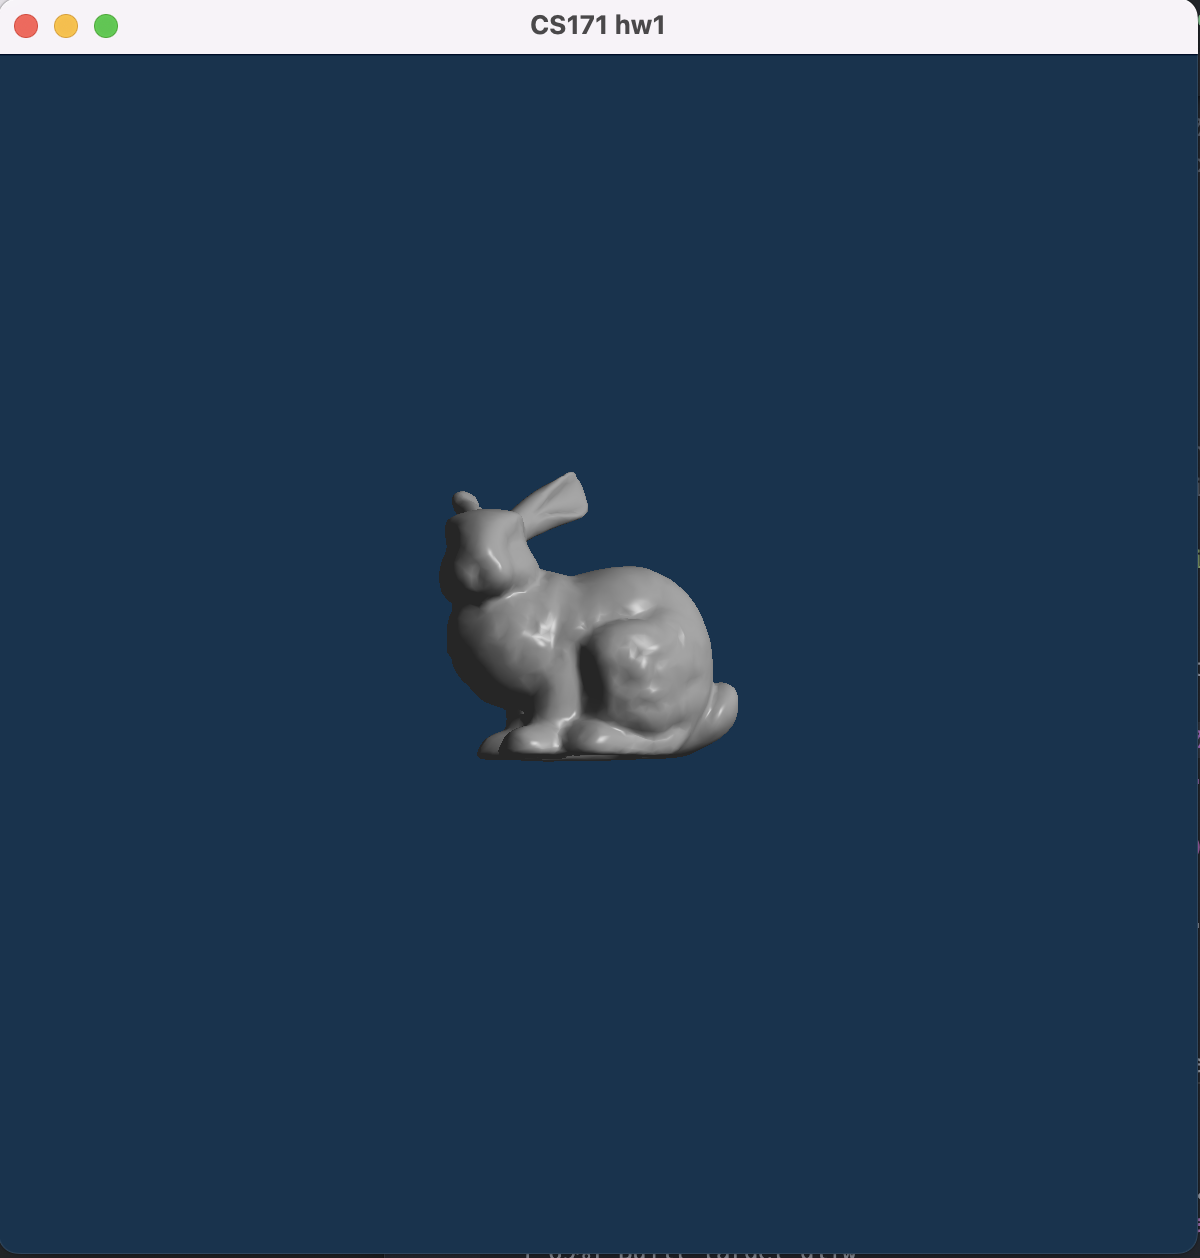
\includegraphics[width=4cm,height=4cm]{bunny_specular.png}
			\caption{ambient, diffuse and specular are implemented}
			\end{figure}
		\item \textbf{attenuation}\\
		Implement attenuation to diffuse and specular to make the model looks more real. Also times to the light color. Here I take the formula in learnopengl:
		$$factor = \frac{1.0}{K_0+K_1*d+K_2*d^2}$$ and multiply it to light color.
		\begin{figure}[h]
			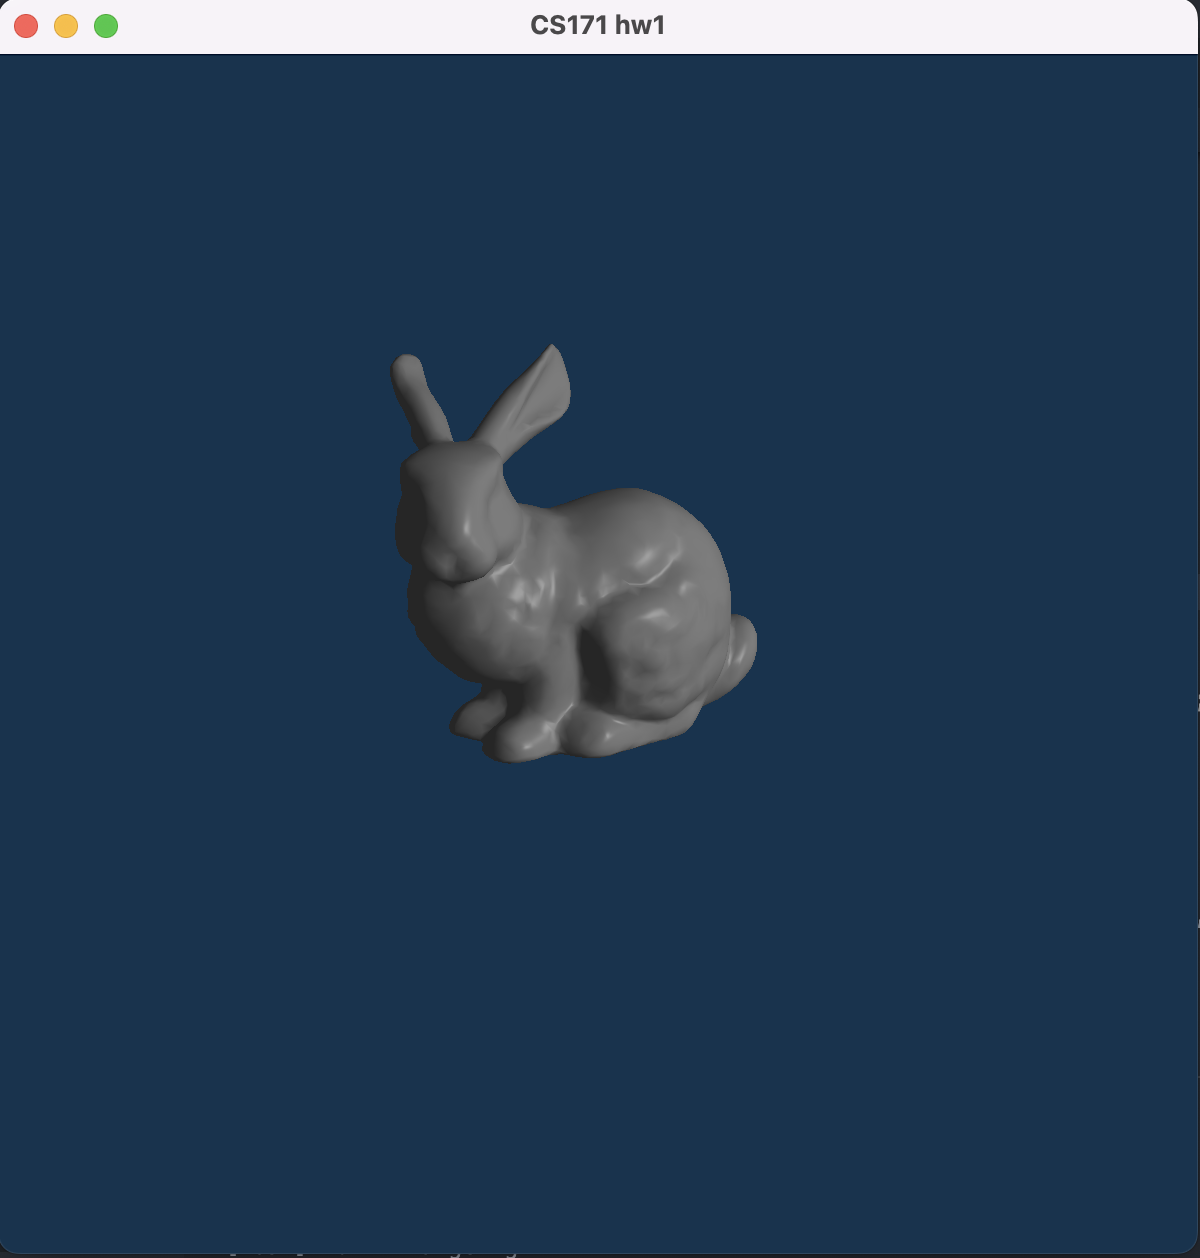
\includegraphics[width=4cm,height=4cm]{bunny_attenuation.png}
			\caption{attenuation is implemented}
			\end{figure}
	\end{enumerate}	
	\item \textbf{Task 3 Camera Control}\\
	I have finished this part actually before task2, according to the teaching sequence on learnopengl. This part requires me to process inputs in every window iteration. We map WASD to the movements of the camera, and the movement and scroll of mouse to the adjust the view direction.
	I implement the speed of view rotations by a factor, which can be obtain be measuring the frame rate, incase the mouse is not too sensitive. Input WASD respectively make the camera position to move up left down and right, simply be adding a vec3 on the camera position.\\
	Considering the rotations of camera, I would prefer to integrate all information into a camera class, solely implemented in camera.h and camera.cpp. Since roll has no use, we can just consider yaw and pitch of the camera, and adjust the camera direction. And as for the zoom or back of camera, we can just move the camera position along the camera direction to realize.
	\item \textbf{Bonus 1 Play with light}\\
	I choose the Carrying a Flashlight (Spot Light) with the camera in bonus 1. I implement the cone spot light, stick it's light position to the camera position, to realize a moving light source just as a flashlight. Cut off the light area from the dark, by calculating the dot product, i.e. comparing dot product is equivalent to comparing the angle from the camera direction, if the angle exceed the cut off range, it would just have ambient light.\\
	\begin{figure}[h]
		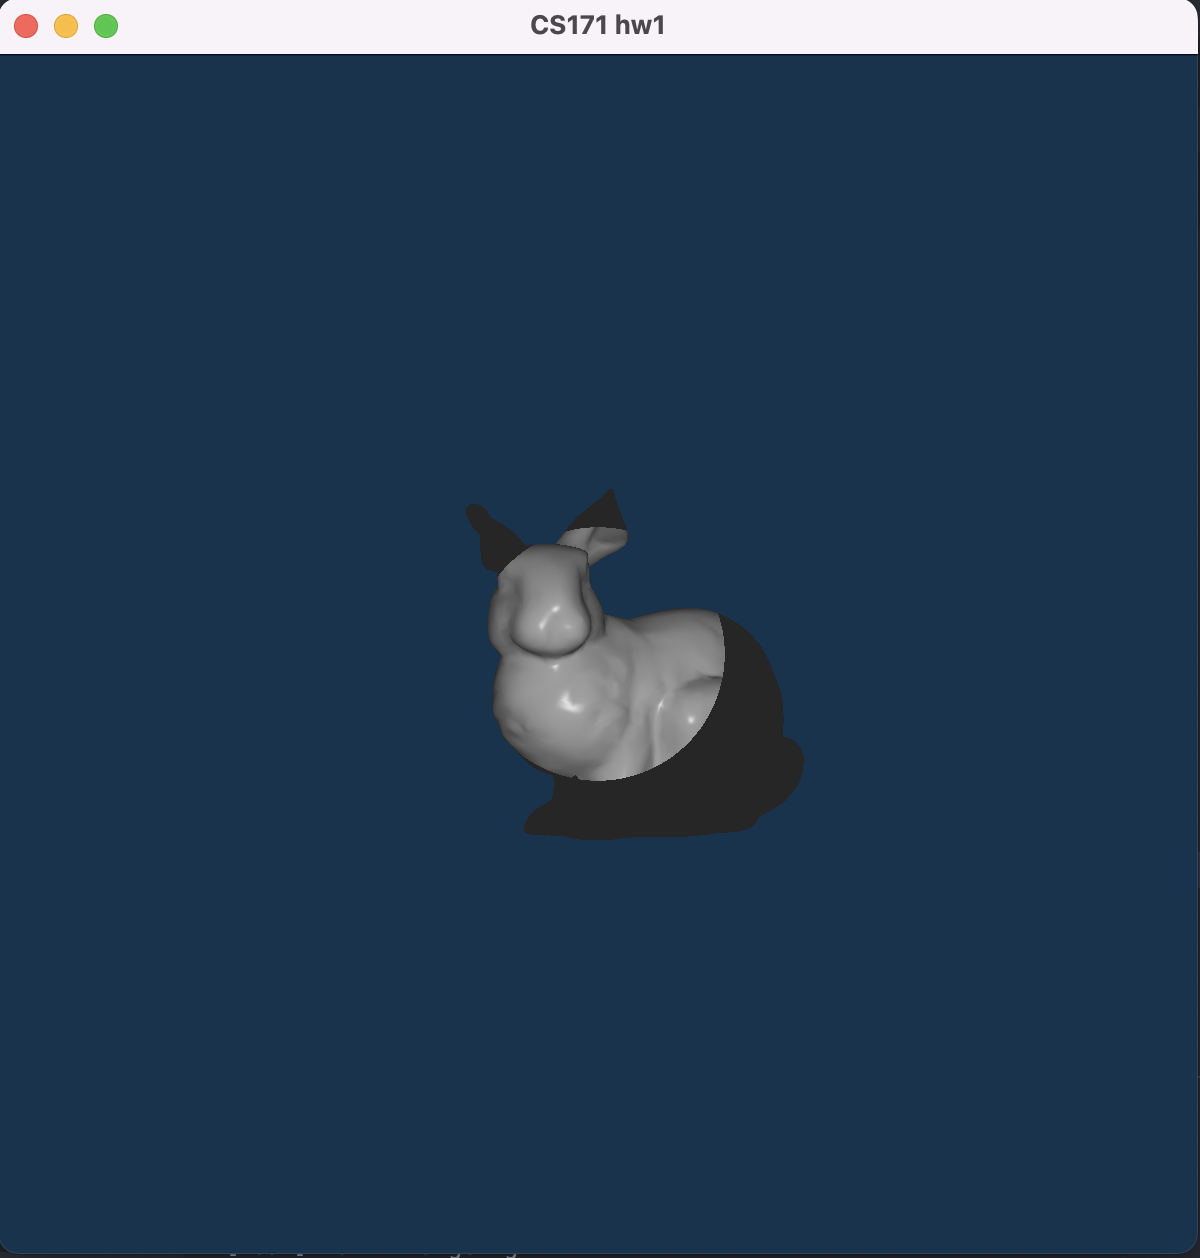
\includegraphics[width=4cm,height=4cm]{bunny_spot.png}
		\caption{spot light is implemented}
		\end{figure}
	But, it looks a little bit wired since the light edge is too sharp. 
	\begin{figure}[h]
		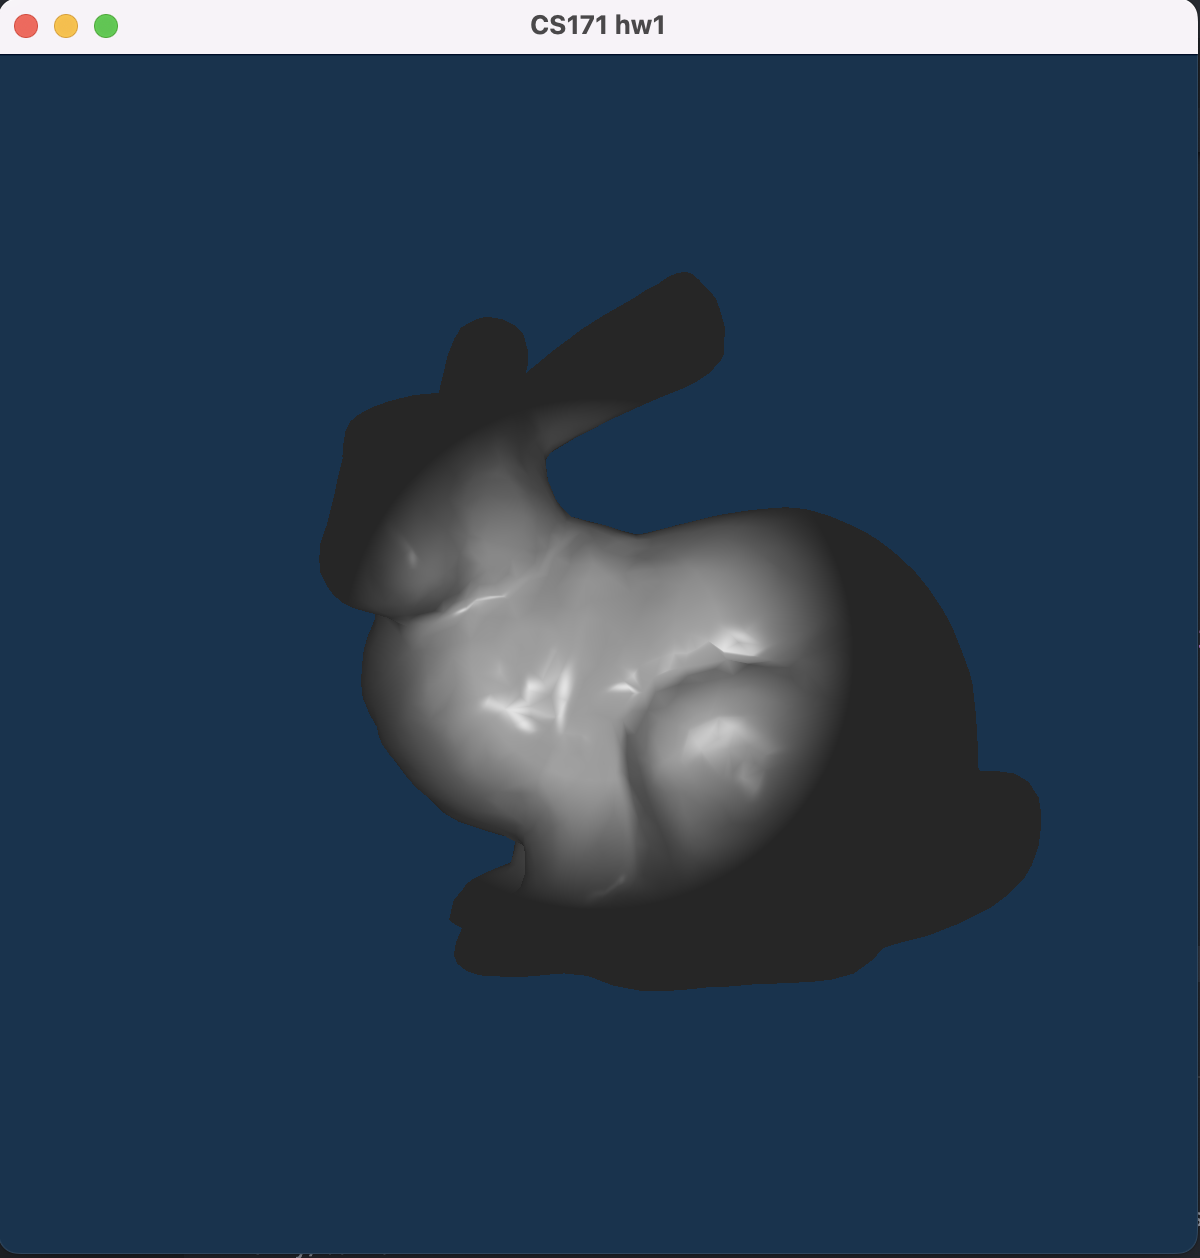
\includegraphics[width=4cm,height=4cm]{bunny_soft.png}
		\caption{soft light is implemented}
	\end{figure}
	Now consider implement a soft light on the edge, by a linear transition on a cutting edge and an outter cutting edge, i.e. the linear transition in the angle, or we can say the linear transition between two dot products. The spot light looks more real now.
	\item \textbf{Bonus 2 Geometry Shader}\\
	I encountered some trouble in this part, since I didn't follow the easy example toturial in learnopengl, directly implement it on the bonus 1 code. The interface is a little bit complicated since I didn't make it too clear.
	After tons of tests to compile all three shaders, and to
	link them correctly, by changing in and out in fragment shader and vertex shader. (mark, here to tip that the struct in fs vs or gs should not be the same as declared in c program, though the language is quite similar to c, but still we should declare directly starting with in and out, I got stucked here.)
	\begin{figure}[h]
		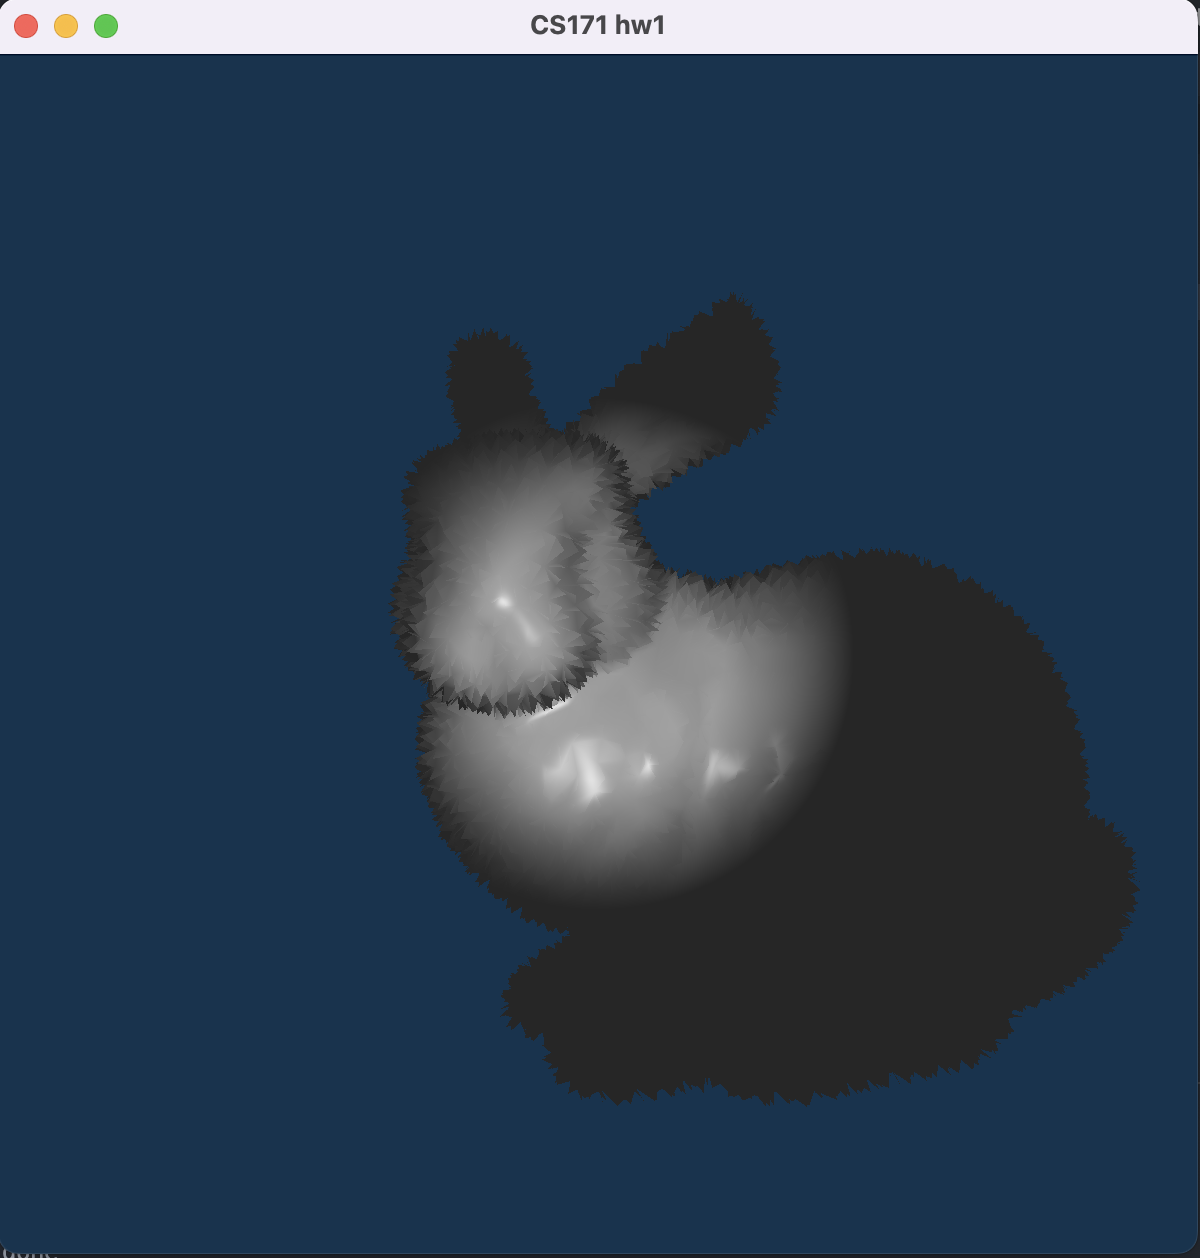
\includegraphics[width=4cm,height=4cm]{bunny_gs.png}
		\caption{gs is implemented}
	\end{figure}
	By visualizing normal vectors, I draw triangle strips using geometry shader, it is actually a tetrahedron on each mesh triangle, and the convex vertex is the normal times a scalar adding to the triangle centroid. 
\end{enumerate}

\section{Results}
% pictures should be in
Pictures are integrated between contexts, and use shellscript "./\_build.sh" after make a build direction to build and run the whole project.

\end{document}
